\documentclass[twoside]{article}
\setlength{\oddsidemargin}{0 in}
\setlength{\evensidemargin}{0 in}
\setlength{\topmargin}{-0.6 in}
\setlength{\textwidth}{6.5 in}
\setlength{\textheight}{8.5 in}
\setlength{\headsep}{0.75 in}
\setlength{\parindent}{0 in}
\setlength{\parskip}{0.1 in}

%
% ADD PACKAGES here:
%
\usepackage[utf8]{inputenc}
\usepackage{amsmath,amsfonts,amssymb,graphicx}
\usepackage[document]{ragged2e}
\usepackage[Euler]{upgreek}
\usepackage{amsthm}

\usepackage[backend=biber]{biblatex}
\addbibresource{ref.bib}

\graphicspath{{./rsc/}{./rsc/pdf/}{./rsc/svg/}}

% Define mathbfit
\DeclareMathAlphabet{\mathbfit}{OML}{cmm}{b}{it}
\DeclareMathAlphabet{\mathbfsf}{\encodingdefault}{\sfdefault}{bx}{n}

% Define operators
\DeclareMathOperator*{\argmax}{arg\,max}
\DeclareMathOperator*{\argmin}{arg\,min}
\DeclareMathOperator*{\minimize}{Minimize}
\DeclareMathOperator*{\maximize}{Maximize}

% Define textbfit
\makeatletter
\DeclareRobustCommand\bfseriesitshape{
  \not@math@alphabet\itshapebfseries\relax
  \fontseries\bfdefault
  \fontshape\itdefault
  \selectfont
}
\makeatother
\DeclareTextFontCommand{\textbfit}{\bfseriesitshape}

%
% The following commands set up the lecnum (lecture number)
% counter and make various numbering schemes work relative
% to the lecture number.
%
\newcounter{lecnum}
\renewcommand{\thepage}{\thelecnum-\arabic{page}}
\renewcommand{\thesection}{\thelecnum.\arabic{section}}
\renewcommand{\theequation}{\thelecnum.\arabic{equation}}
\renewcommand{\thefigure}{\thelecnum.\arabic{figure}}
\renewcommand{\thetable}{\thelecnum.\arabic{table}}

%
% Narrower margin
%
\def\changemargin#1#2{\list{}{\rightmargin#2\leftmargin#1}\item[]}
\let\endchangemargin=\endlist
%
% The following macro is used to generate the header.
%
\newcommand{\lecture}[4]{
  \pagestyle{myheadings}
  \thispagestyle{plain}
  \newpage
  \setcounter{lecnum}{#1}
  \setcounter{page}{1}
  \noindent
  \begin{center}
    \framebox{
      \vbox{
        \vspace{2mm}
        \hbox to 6.28in { {\bf MAT2013: Probability and Statistics~\cite{IPSUR-2010}~\cite{RP-Babatunde-2009} \hfill Spring 2017} }
        \vspace{4mm}
        \hbox to 6.28in { {\Large \hfill Lecture #1: #2  \hfill} }
        \vspace{2mm}
        \hbox to 6.28in { {\it Lecturer: #3 \hfill Scribes: #4\/} }
        \vspace{2mm}
      }
    }
  \end{center}
  \markboth{Lecture #1: #2}{Lecture #1: #2}
  {\textbf{Scribes}}: {
    Jisung Lim,
    \textit{B.S. Candidate of Industrial Engineering
    in Yonsei University, South Korea.}
  }

  {\textbf{Disclaimer}}: {
    \textit{These notes have not been subjected to the
    usual scrutiny reserved for formal publications.  They may be distributed
    outside this class only with the permission of the Instructor.}
  }
  \vspace*{4mm}
}
%
% Convention for citations is authors' initials followed by the year.
% For example, to cite a paper by Leighton and Maggs you would type
% \cite{LM89}, and to cite a paper by Strassen you would type \cite{S69}.
% (To avoid bibliography problems, for now we redefine the \cite command.)
% Also commands that create a suitable format for the reference list.
%\renewcommand{\cite}[1]{[#1]}
% \def\beginrefs{\begin{list}%
%         {[\arabic{equation}]}{\usecounter{equation}
%          \setlength{\leftmargin}{2.0truecm}\setlength{\labelsep}{0.4truecm}%
%          \setlength{\labelwidth}{1.6truecm}}}
% \def\endrefs{\end{list}}
% \def\bibentry#1{\item[\hbox{[#1]}]}

%Use this command for a figure; it puts a figure in wherever you want it.
%usage: \fig{NUMBER}{SPACE-IN-INCHES}{CAPTION}
\newcommand{\fig}[3]{
			\vspace{#2}
			\begin{center}
			Figure \thelecnum.#1:~#3
			\end{center}
	}

% Use these for theorems, lemmas, proofs, etc.

\theoremstyle{definition}
\newtheorem{definition}{Definition}[section]
\newtheorem{theorem}[definition]{Theorem}
\newtheorem{lemma}{Lemma}[definition]
\newtheorem{proposition}{Proposition}[definition]
\newtheorem{claim}{Claim}[definition]
\newtheorem{corollary}{Corollary}[definition]

\theoremstyle{remark}
\newtheorem{properties}{Properties}[definition]
\newtheorem{question}{Question in Lecture}[lecnum]
\newtheorem{example}{Example}[lecnum]

\newenvironment{prf}{{\bf Proof:}}{\hfill\rule{2mm}{2mm}}
\newenvironment{sol}{{\bf Solution:}}{\hfill\rule{2mm}{2mm}}
\newenvironment{skt}{{\bf Sketch:}}
% **** IF YOU WANT TO DEFINE ADDITIONAL MACROS FOR YOURSELF, PUT THEM HERE:

\newcommand\E{\mathbb{E}}

\begin{document}
%FILL IN THE RIGHT INFO.
%\lecture{**LECTURE-NUMBER**}{**DATE**}{**LECTURER**}{**SCRIBE**}
\lecture{1}{Introduction, Basics of Probability}{Jae Guk, Kim}{Jisung Lim}
%\footnotetext{These notes are partially based on those of Nigel Mansell.}

% **** YOUR NOTES GO HERE:


\section{Why do we have to study probabilty?}

\textbfit{To model the random phenomena in the mathematical framework with consistency.}

\section{How to model the random experiment?}
\subsection{Identifying Sample Space}
\begin{definition}{\bf Random Experiment} \\
  A \textbf{random experiment} is one whose outcome is determined by chance.
  The result is unknown, until we observe the outcome.
\end{definition}
(ex) Tossing a coin, rolling a dice.


\begin{definition}{\bf Sample Space} \\
  For a random experiment, the set of all possible outcomes of it is called
  \textbf{the sample space} $S$ of \textbf{the random experiment}.
\end{definition}

ex. Coin-tossing
\\ Sample space: $S = \{\mathrm{HEAD}, \mathrm{TAIL}\}$

\begin{definition}{\bf Event} \\
  An event $A$ is a subset of the sample space $S$.
\end{definition}

ex. Rolling a dice
\\ Sample space: $S = \{1,2,3,4,5,6\}$, Event: $A_0 = \emptyset$, \ldots, \{1, 3\}

\begin{definition}{\bf Mutually Exclusive} \\
  We say that a bunch of events $A_1,A_2,\ldots$ are \textbf{mutually exclusive}
  if $$A_i \cap A_j = \emptyset \quad \textrm{for} \quad i \neq j$$
\end{definition}

ex. Coin tossing
\\ Sample space: $A_1 = \{\mathrm{HEAD}\}, A_2 = \{\mathrm{TAIL}\}$

\clearpage

\subsection{Assigning a probability to each elements in sample space}

\subsubsection{What do we mean when we say ``the probability of Heads,'' $P(\textrm{Head})$?}

\textbf{Answer 1. Relative Frequency Approach (Bernoulli trial)}
\begin{itemize}
  \item This approach states that the way to determine $P(\textrm{Head})$ is
  to flip the coin repeatedly in exactly the same way each time. \\
  Then, a good approximation to $P(\textrm{Head})$ will be
  $$P(\textrm{Head}) \simeq
  \frac{\textrm{(number of observed heads)}}{\textrm{(total \# of flips)}}$$

  \item A justification for this approach comes from \textbf{the law of large numbers}.
\end{itemize}

\begin{theorem}
  \textbf{The law of large number (LLN)}.\\
  \begin{equation}
    \frac{S_n}{n} \rightarrow P(A) \quad as \quad n \rightarrow \infty
  \end{equation}
  where
  \begin{equation}
    \begin{split}
      A   &: \textrm{event} \\
      n   &: \textrm{the \# of conducted experiments} \\
      S_n &: \textrm{the \# of times that A occurred in the n experiments} \\
    \end{split}
  \end{equation}
\end{theorem}

\textbf{So, is there any problem in using Relative Frequency Approach to calculate the probability?} \\
\begin{itemize}
  \item It is just a \textrm{long-run} approximation: It requires the large number
        of experiments!
  \item Is it possible to compute the probability of you getting A in this class?
\end{itemize}

\textbf{Answer 2. The Subjective Approach (Bayesian)}
\begin{itemize}
  \item This approach interprets probability as the experimenter's
    \textbf{degree of belief} that an event of interest will occur.

  \item Ex) What is the probability that she/he likes me? \\
    To answer this questions, we refer to the use of intuition,
    personal belief, and other direct/indirect informations.
    this is the subjective definition of probability.
\end{itemize}

\textbf{\# Brief insight} \\
In most cases of random phenomena of science and engineering, the relative
frequency interpretation of probability is the operative one. (More info, see appendix.)

\textbf{Anyway} \\
In consequence, modeling a random phenomena is a process of identifying a
sample space $S$ and assigning probabilities to all the events $A_1,A_2,\ldots$
of the sample space $S$.

\clearpage

\subsubsection{Probability Model}
The mathematical description of a random phenomenon consisting of two parts:
\begin{itemize}
  \item a sample space S
  \item a way of assigning probabilities.
\end{itemize}

It will be tricky as you expect but there is very obvious case in giving
probabilities.

We used coin-tossing example to explain the relative frequency interpretation
of probability. However, it is obvious to select a model for it,
\begin{equation}
  P(\textrm{Head}) = \frac{1}{2}, P(\textrm{Tail}) = \frac{1}{2}
\end{equation}
provided that the coin is well-balanced.

In general, it is good to assign a probability to an event in Equally Likely Model
through
\begin{equation}
  P(A_i) = \frac{1}{N} \quad \forall i \in \{1,\ldots,N\}
\end{equation}

\section{The viewpoint: Probability Measure (function)}

\subsection{Proability Function and its Properties}
Now, we consider probability as a function from a collection of events $\mathcal{P}(S)$
to the real-valued interval $\mathbb{R} \in [0, 1]$, which is called probability measure.
A probability function is a rule that associates with each event $A$ of the
sample space $S$. A unique quantity $P(A) = a$, called the probability of $A$.

\begin{definition}
  Any probability function $P$ satisfies the following Kolmogorov Axioms:
  \begin{enumerate}
    \item $P(A) \geq 0$ for any event $A \subseteq S$
    \item $P(S) = 1$
    \item If the countable events $A_1, A_2, A_3, \ldots$ are mutually exclusive,
          then
          $$
          P(\cup_{i=1}^{\infty} A_i) = \sum_{i=1}^{\infty} P(A_i)
          $$
  \end{enumerate}
\end{definition}

\begin{properties}
  Let $P$ be the probability function which satisfies the Kolmogorv Axioms:
  \begin{enumerate}
    \item $P(\emptyset) = 0$ \\
    \begin{proof}
      Hint: Let assume $A_i = \emptyset \quad \forall i \in \mathbb{N}$
    \end{proof}

    \item For every finite $A_1, A_2, A_3,\ldots, A_m$ of mutually exclusive
          events $A_i \subseteq S$, we have
          \begin{equation}
            P\left(\cup_{i=1}^{m} A_i\right) = \sum_{i=1}^{m} P(A_i)
          \end{equation}
          \begin{proof}
            Hint: $B_i = A_i \forall i = \{ 1,\ldots, m \}$ and $B_j = \emptyset \forall i = \{ m+1,m+2,\ldots \}$
          \end{proof}

    \item $P(A^C) =  1 - P(A)$ \\
    \begin{proof}
      Hint: $1 = P(S) = P(A \cup A^C) = P(A) + P(A^C)$
    \end{proof}

    \item If $A \subset B$, then $P(A) \leq P(B)$ \\
    \begin{proof}
      Hint: $B=A \cup (B \cap A^C)$
    \end{proof}

    \item $\forall A \subseteq S,\, 0 \leq P(A) \leq 1$ \\
    \begin{proof}
      \begin{enumerate}
        \item $0 \leq P(A)$ \\
        Hint: Axiom 1.
        \item $P(A) \leq 1$ \\
        Hint: Axiom 2: $P(S) = 1$, $A \subset S$, and property 4.
      \end{enumerate}
      By (a) and (b), the proposition is true.
    \end{proof}

    \item (Additive rule) $P(A \cup B) = P(A) + P(B) - P(A \cap B)$ \\
    \begin{skt}
      Sketch diagram to grasp intution for solving the problem.
    \end{skt}
    \begin{prf}
      Hint: $(A \cap B^C) \cup (A \cap B) \cup (A^C \cap B)$
    \end{prf}

    \item (Total probability) Let $B_1, B_2, \ldots, B_n$ be mutually exclusive
          and exhaustive, then $P(A) = P(A \cap B_1) + P(A \cap B_2) + \cdots + P(A \cap B_n)$. \\
    \begin{prf} \\
      (Mutually exclusive): We say that a bunch of events $B_1, B_2, \ldots$ are
      mutually exclusive if
      $$ B_i \cap B_j = \emptyset \quad \textrm{for} \quad i \neq j $$
      (Collectively exhaustive): We say that a bunch of events $B_1, B_2, \ldots$ are
      collectively exhaustive if
      $$ \cup_{i=1}^{\infty} B_i = S $$
      Hint: $P(A) = P(A \cap S)
             = P(A \cap (\cup_{i=1}^{\infty} B_i))
             = P(\cup_{i=1}^{\infty}(A \cap B_i))
             = \sum_{i=1}^{\infty} P(A \cap B_i)$
    \end{prf}
  \end{enumerate}
\end{properties}

\subsection{Conditional Probability}

Now, we want to deal with a situation like, what is the probability of $A$ occurring
given knowledge that $B$ has occured?

\begin{example}
  Consider a full deck of 52 cards. (1, 2, 3, 4, \ldots, 13). Select two cards
  successively.
  $$ A = \{ \textrm{first card drawn is an 1} \} $$
  $$ B = \{ \textrm{second card drawn is an 1} \} $$

  \begin{sol}
    By definition, our sample space is given by,
    $$
    S = \{ (1A,1B), (1A,1C), (1A, 1D), \ldots, (1A, 13D), \ldots, (13B, 13D), (13C, 13D) \}
    $$
    which has the number of cases $n(S) = 52 \times 51$. Before we evaluate some
    probabilities, let's introduce a basic counting principle called additive rule
    and product rule.

    \begin{definition}
      {\bf The rule of sum} \\
      If a first task can be performed in $m$ ways, while a second task can be performed
      in $n$ ways, and the \textbf{two tasks cannot be performed simultaneously}, then
      performing either task can be accomplished in any one of $m+n$ ways.
    \end{definition}
    \begin{definition}
      {\bf The rule of product} \\
      If a procedure can be broken down into first and second stages, and if there are
      $m$ possible outcomes for the first stage and if, for each of these outcomes,
      there are $n$ possible outcomes for the second stage, then the total procedure can
      be carried out, in the designated order, in $m \cdot n$ ways.
    \end{definition}

    Then we can calculate the
    probability of $A$ and $B$, respectively, which is given by
    $$
    P(A) = \frac{4}{52} \frac{51}{51} = \frac{4}{52}
    $$
    and
    $$
    P(B) = \frac{4}{52} \frac{3}{51} + \frac{48}{52} \frac{4}{51}.
    $$
    \\[1.5\baselineskip]
    Also we can find joint probability of $A$ and $B$, which is given by
    $$
    P(A \cap B) = \frac{4 \times 3}{52 \times 51}.
    $$
    \\[1.5\baselineskip]
    Now, let us consider the conditional probability, the probability of $A$ occrring
    given knowledge that $B$ has occured, which is given by
    $$
    P(B|A) = \frac{3}{51}.
    $$
  \end{sol}
\end{example}

In the latest example, our evalution process of the probabilities of various events
seems to strongly depend on the knoweledge of the specific situation. Now, we
want to generalize this evaluation process into systematic framework to solve
similar problems without exploiting any situation-based knoweledge.

\begin{skt}
  First, we may consider roughly (or intuitively) the reduced sample space
  from $S$ to $B$.
  \begin{figure}[h]
    \centering
    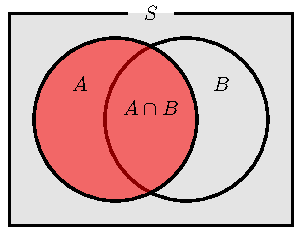
\includegraphics[height=4cm]{conditional_a.pdf}
    \caption{conditional distribution}
  \end{figure}


  Then, we can evaluate the conditional distribution
  $$
  P[B|A] = \frac{12 / (52 \times 51)}{4 / 52} = \frac{3}{51}.
  $$
\end{skt}


Now, we will define the conditional probablity more precisely, and rigorously
as follows:

\begin{definition}
  Let $A$, $B$ be events, $P(A) > 0$. The conditional probability of $B$ given $A$
  is
  \begin{equation}
    P[B|A] = \frac{P(A \cap B)}{P(A)}
  \end{equation}
\end{definition}

\begin{theorem}
  For any fixed event $A$ with $P(A)>0$
  \begin{enumerate}
    \item $P[B|A] \geq 0 \quad \forall B \subset S$
    \item $P[S|A] = 1$
    \item If $B_1, B_2, B_3, \ldots$ are disjoint events, then
    $$
    P(\bigcup_{i=1}^{\infty} B_i | A) = \sum_{i=1}^{\infty} P(B_i | A)
    $$
  \end{enumerate}
  That is, the conditional probability $P(\cdot|A)$ is also a probability function.
\end{theorem}

\begin{properties}
  Then the following are immediate, for any events $A, B, C$ with $P(A) > 0$,
  \begin{enumerate}
    \item $P(B^C|A) = 1 - P(B|A)$
    \item if $B \subset C$, then $P(B|A) \leq P(C|A)$
    \item $P((B \cup C) | A) = P(B|A) + P(C|A) - P((B \cap C) | A)$
    \item (The mulitplication Rule) For any two events $A$ and $B$,
    $$
    P(A \cap B) = P(A) P(B|A)
    $$
    And more generally, for events $A_1, A_2, \ldots, A_n$
    $$
    P(A_1 \cap A_2 \cap A_3 \cap \cdots \cap A_n)
    =P(A_1)P(A_2|A_1)P(A_3|A_1 \cap A_2) \cdots P(A_n|A_1 \cap A_2 \cap \cdots \cap A_{n-1})
    $$

  \end{enumerate}
\end{properties}

\begin{example}{\bf Card selection} \\
  Let's calculate the probability of two sequential outcomes being both 1.
  First, we can count every cases using our knoweledge about the situation,
  which is given by
  $$
  P(\textrm{both 1}) = P(A \cap B) = \frac{4 \times 3}{52 \times 51}
  $$
  But, we want to evaluate the probability by exploiting mathematical framework,
  not using our situation-based knoweledge and intuition.
  $$
  P(B \cap A) = P(A) P(B|A) = \frac{4}{52} \cdot  \frac{12 / (52 \times 51)}{4 / 52}
  $$
\end{example}

\begin{example}{\bf Red-Green Ball} \\
  There is an urn with 10 balls inside: 7 red balls and 3 green balls. We will
  draw three balls sequentially from the urn, and our event of interest is the
  case where all three balls are red. Then, we can divide the event into three
  sub event as follows:
  \begin{itemize}
    \item $A_1 = \{\textrm{1st ball is red}\}$
    \item $A_2 = \{\textrm{2nd ball is red}\}$
    \item $A_3 = \{\textrm{3rd ball is red}\}$
  \end{itemize}
  And we can evaluate the probability of our event of interest systematically:
  $$
  P(\textrm{All 3 balls are red}) = P(A \cap B \cap C) = P(A) P(B|A) P(C|B \cap A)
  $$
\end{example}

\clearpage
\subsection{Independence}
Given events $A$ and $B$, the situation where knowledge that $B$ has occurred in
no way changes the probability that $A$ will occur. A proper way to represent it
would be
\begin{equation}
  P(A|B) = P(A) \quad \textrm{where} \quad P(B) > 0
\end{equation}

More specifically, consider you toss a coin twice, then sample space $S$ is given by
$$
S = \{ HH, HT, TH, TT \}
$$
and we assume the model has probability with equally likely event,
$$
P(HH) = P(HT) = P(TH) = P(TT) = 1/4
$$
Now, lets evaluate the following probabilities
$$
P(\textrm{2nd toss is H} | \textrm{1st toss is H})
= \frac{P(\textrm{both H})}{P(\textrm{1st toss is H})}
= \frac{1/4}{1/2} = \frac{2}{4} = \frac{1}{2}
$$
$$
P(\textrm{2nd toss is H}) = \frac{P(\textrm{2nd toss is H})}{P(S)}
= \frac{2}{4} = \frac{1}{2}
$$
$$
P(\textrm{2nd toss is H} | \textrm{1st toss is H}) = P(\textrm{2nd toss is H})
$$
This means that the information that ``the first toss is H'' has nothing to do with
the probability that ``the second toss is H''. That is, the coin deos not remenber
the result of the first toss.

\begin{question}
  Why coin tossing example can be used in numerous examples? \\
  \textit{ANS.} Symmetric property of coin tossing.
\end{question}

\begin{definition}
  Events A and B are said to be independent if
  \begin{equation}
    P(A \cap B) = P(A)P(B)
  \end{equation}
  Otherwise, the events are said to be dependent.
\end{definition}

\begin{theorem}
  If the events $A$ and $B$ are independent, then
  \begin{enumerate}
    \item $A$ and $B^C$ are independent \\
    \begin{skt}
      w.t.s: $P(A^C \cap B) = P(A^C) P(B) \quad \cdots \quad (1)$
    \end{skt}
    \begin{prf}\\
      Let $P(B) > 0$, by multiplication rule, (1) becomes
      $$
      P(A^C \cap B) = P(B) P(A^C|B) \quad \cdots \quad (2)
      $$
      Since the conditional probability $P(\cdot|B)$ is also the probability
      function, by property of complement set,
      $$
      P(B) P(A^C|B) =  P(B)(1- P(A|B)) \quad \cdots \quad (3)
      $$
      Since $A$ and $B$ are independent, then
      $$
      P(B)(1 - P(A))
      $$
      By property of probability function
      $$
      P(B)(A^C)
      $$
    \end{prf}
    \item $A^C$ and $B$ are independent
    \item $A^C$ and $B^C$ are independent
  \end{enumerate}
\end{theorem}

\clearpage
What if there are more than two events of interest?
\begin{definition}
  Any collection of events ${\{A_i\}}_{i \in I}$ is independent if for every finite
  subset $J \subset I$, one has
  \begin{equation}
    P(\cap_{i \in J} A_i) = \prod_{i \in J} P(A_i)
  \end{equation}
\end{definition}

It is often called to be mutually independent.

\textbf{Note.} if events are ${\{A_i\}}_{i \in I}$ is independent, they pairwise
independent but the converse is false. (${\{A_i\}}_{i \in I}$ are pairwise
independent if $A_i$ and $A_j$ are independent for all $i, j$ with $i \neq j$)

\begin{example}
  Let the sample space $S = \{1,2,3,4\}$ and each single event is equally likely
  probable $P(i) = 1/4 \quad \forall i \in \{ 1, 2, 3, 4 \}$. Then we can construct
  a collection of events $\mathbb{C} = {\{ A, B, C \}}$, in which each event is
  given by:
  $$
  A = \{ 1, 2 \}, B = \{ 1, 3 \}, C = \{ 2, 3 \}
  $$

  Let us evaluate the probability of pair of each event, which is given by
  \begin{itemize}
    \item $P(A \cap B) = P(\{ 1 \}) = 1/4 = (1/2)(1/2) = P(A)P(B)$
    \item $P(B \cap C) = P(\{ 3 \}) = 1/4 = (1/2)(1/2) = P(B)P(C)$
    \item $P(A \cap C) = P(\{ 2 \}) = 1/4 = (1/2)(1/2) = P(A)P(C)$
  \end{itemize}
  which implies pairwise independent.

  But, if we evaluate the probability of $A \cap B \cap C$, then
  $$
  P(A \cap B \cap C) = P(\emptyset) = 0.
  $$
  and since $P(A)P(B)P(C) = 1/8$, then
  $$
  P(A \cap B \cap C) \neq P(A)P(B)P(C),
  $$
  which implies the collection of events ${\{ A, B, C \}}$ is not mutually independent.
\end{example}

\subsubsection{Independence vs. exclusive, pairwisely vs. mutually}
So far, we've discussed about difference between \textit{pairwisely} and \textit{mutually},
in the context of \textbf{independence}. As we've seen before, the notion of
\textit{pairwisely} and \textit{mutually} was introduced when we had discussed
about \textbf{exclusive}. You may be confused between two different concepts.
Let's take an example of exclusive to separate two different concept---independence
and exclusive, in the perspective of \textit{pairwisely} and \textit{mutually}.

First, for our example, let us define the \textit{partition}, which satisfies
two properties, mutually exclusive and collectively exhaustive.
\begin{definition}
  A collection of events ${\{ E_n \}}_{n \in \mathbb{N}}$ is called a partition
  of $S$ if they are pairwise disjoint,
  $$
  P(E_n) > 0, \cup_{n\in \mathbb{N}}(E_n) = S
  $$
\end{definition}

\begin{example}
  {Does partitions have mutually exclusive property? Prove your claim.}
\end{example}
\begin{prf}
  {\it Hint.} A collection of sets are pairwise disjoint implies the collection
  is mutually exclusive.
\end{prf}

\clearpage
\begin{theorem}{\bf Bayes' Theorem}\\
  Let ${E_n}$ be a finite or countable partition of $S$, and suppose $P(A) > 0$,
  then
  \begin{equation}
    P(E_n | A) = \frac{P(A|E_n) P(E_n)}{\sum_m P(A|E_m)P(E_m)}
  \end{equation}
\end{theorem}
\begin{skt}
  $$
  P(E_n|A)
  = \frac{P(E_n \cap A)}{P(A)} \frac{P(E_n)}{P(E_n)}
  = \frac{P(A|E_n) P(E_n)}{P(A)}
  = \frac{P(A|E_n) P(E_n)}{\sum_m P(A \cap E_m)}
  $$
\end{skt}
\begin{prf}
  \textit{D.I.Y.}
\end{prf}
\\[2.0\baselineskip]

\begin{example}
  p.103 (This solution may be \textit{WRONG} because the scriber refers to
  additional material. There are some concepts and contents that are not
  mentioned in the lecture, so I've included references to that contents.)
  \\[1.5\baselineskip]
\end{example}
\begin{skt}
  {\bf Modeling the random phenomena} \\
  {\bf 1. Specify our random experiment.} \\
  Select one of the documents from the cabinet. We may find two kinds of
  information in the experiment.
  \begin{itemize}
    \setlength\itemsep{0.2em}
    \item ``Who filed this document?''
    \item ``Is document misplaced?''
  \end{itemize}
  The possible outcomes for first question is one of Moe, Larry, and Curly and
  the possible outcomes for second question is that the document is misfiled or
  not. Like this case, if we have more than one kind of `outcomes of interest,'
  we may construct multiple sample space for each kind of outcomes~\cite{wiki:SampleSpace}.
  Hence, we can construct two sample space for each question, which is given by
  $$
  S_1 = {\{ m, l, c \}},\, S_2 = {\{ a, \bar{a} \}}
  $$
  where $m$, $l$ and $c$ stands for Moe, Larry, and Curly for the first question,
  respectively, and $a$ implies that the document is misplaced, $\bar{a}$ implies
  not.

  {\bf 2. Construct our sample space}\\
  From here, we can define our sample space as the Cartesian product of the two
  sample spaces noted above:
  $$
  S = S_1 \times S_2 = {\{(m,a), (l,a), (c,a), (m,\bar{a}), (l,\bar{a}), (c,\bar{a}) \}}
  $$

  {\bf 3. Determine our events of interest}\\
  Our events of interest can be determined based on our previous two questions
  and their associated answers. Hence our events are determined as follows
  \begin{itemize}
    \setlength\itemsep{0.2em}
    \item $M = {\textrm{Moe filed the document}} = {\{(m,a), (m,\bar{a})\}}$
    \item $L = {\textrm{Larry filed the document}} = {\{(l,a), (l,\bar{a})\}}$
    \item $C = {\textrm{Curly filed the document}} = {\{(c,a), (c,\bar{a})\}}$
  \end{itemize}
  and
  \begin{itemize}
    \setlength\itemsep{0.2em}
    \item $A = {\textrm{The file is miss classified}} = {\{(m,a), (l,a), (c,a)\}}$
  \end{itemize}
  From this setting, we can sketch the diagram as follows:
  \\[3.0\baselineskip]
  \begin{figure}[h]
    \centering
    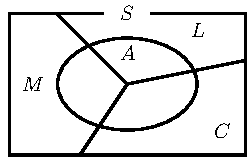
\includegraphics[height=3.5cm]{mlc_file.pdf}
    \caption{sample space diagram}
  \end{figure}

  {\bf 4. Assign probabilities to each event} \\
  First, picking up any file from the cabinet is assumed to occur equally likely.
  From this assumption, we can evaluate the probability of each event based on
  counting. (e.g. $P(M)=n(M)/n(S)$.) Because of the assumption of same labor
  efficiency, we can say that each probability is proportional to the workload
  on each assistants. From the given information about the workload, we can
  assign probabilities to each event, given by
  $$
  P(M) = \frac{6}{10}, P(L) = \frac{3}{10}, P(C) = \frac{1}{10}
  $$

  And also we have another infomration called `Misfile Rate', the rate of misfiling
  of each assistant when the documents was filed by that assistant. By the
  definition, Misfile Rate can be viewed as a conditional probability as follows
  $$
  P(A|M) = 0.003, P(A|L) = 0.007, P(A|L) = 0.010
  $$
  which implies the probability of the file is miss classified, when the knowledge
  that the file is classified by Moe, Larry, or Curly, respectively, is given.

  {\bf 5. Properties of events} \\
  Since any two person cannot classify same file simultaneously, each event $M$,
  $L$ and $C$ is \textbf{mutually exclusive}. Since no one classifies files except
  for those three assistants: Moe, Larry, and Curly, then each event $M$, $L$,
  and $C$ is \textbf{collectively exhaustive}. Hence, by definition, a collection
  of those three events is a partition of sample space $S$.
\end{skt}
\begin{sol}
  Use the Bayes' rule. Find $P(M|A), P(L|A), P(C|A)$. \textit{D.I.Y.}
\end{sol}


\clearpage
\subsection{Counting Methods}
In the equally likely model,
$$
P(A) = \frac{\textrm{(\# of A)}}{\textrm{(\# of S)}}
$$
Thus, it is important to count outcomes in the event of interest.
\begin{definition}
  {\bf Multiplication Principle} \\
  If an experiment is composed of $k$ successive steps which may be performed
  in $n_1, n_2, \ldots, n_k$ distinct ways, respectively, then the experiment
  may be performed in $n_1 \cdot n_2 \cdots n_k$ distinct ways.
\end{definition}

\begin{theorem}
  Every counting problem can be substituted with $k$ balls $n$ bins problem.
  \begin{itemize}
    \item {\bf Ordered sample} \\
    The number of ways in which one may select an ordered sample of $k$ subjects
    from a population that has $n$ distinguishable members is
    \begin{enumerate}
      \item $n(n-1)(n-2)\cdots(n-k+1)$ if sampling is done without replacement.
      \item $n^k$ if sampling is done with replacement.
    \end{enumerate}
    \item {\bf Unordered sample} \\
    The number of ways in which one may select an unordered sample of $k$ subjects
    from a population that has $n$ distinguishable members is
    \begin{enumerate}
      \item $\binom{n}{k}$ if sampling is done without replacement.
      \item $\binom{n+k-1}{n-1} = \binom{n+k-1}{k}$ if sampling is done without replacement.
    \end{enumerate}
  \end{itemize}
\end{theorem}


\begin{example}
  Take a coin and flip it 7 times. How many sequences of Heads and Tails are possible?\\
  \textit{ANS:} 7 balls to 2 bins.
\end{example}
\begin{example}
  We rent five videos, we want to see three movies in specific order.\\
  \textit{ANS:} 3 balls to 5 0--1 bins.
\end{example}


\section{Appendix}
\subsection{Diffrence between Relative Frequency Approach and Subjective Approach}
\begin{itemize}
  \item Relative Frequency Approach (Frequentist)
  \begin{enumerate}
    \item ”Probabilities represent long run frequencies of events.”
    \item Computationally inexpensive relatively.
    \item Do not use subjective information.
    \item But there exist some limitations in performance.
  \end{enumerate}
  \item The Subjective Approach (Bayesian)
  \begin{enumerate}
    \item ”Probability is used to quatify our uncertainty about something or precisely degree of belief.”
    \item Computationally expensive, since we need to compute all the distribution.
    \item Use subjective information.
    \item But the performance is better especially in high dimension.
  \end{enumerate}
\end{itemize}

\subsection{Unordered Sample with Replacement}
Consider ``unordered sample with replacement'' case and let's develope the logic.
Let's consider it with intuition. Assume $k = 2$, then there are two possible
cases,
\begin{itemize}
  \setlength\itemsep{0.0em}
  \item If two balls are in distinct bins, then $\frac{n(n-1)}{2!}$.
  \item If two balls are in the same bin, then $n$.
\end{itemize}
So,
$$
\frac{n(n-1)}{2} + n = \frac{n(n+1)}{2}
$$

What if $k = 3$?
\begin{itemize}
  \setlength\itemsep{0.0em}
  \item If three balls are in three distinct bins, then \ldots.
  \item If three balls are in two distinct bins, then \ldots.
  \item If three balls are in the same bin, then \ldots.
\end{itemize}

What if $k = k_0$?
\begin{itemize}
  \setlength\itemsep{0.0em}
  \item If $k_0$ balls are in $k_0$ distinct bins, then \ldots.
  \item If $k_0$ balls are in $k_0 - 1$ distinct bins, then \ldots.
  \item If $k_0$ balls are in $k_0 - 2$ distinct bins, then \ldots.
  \\ $\cdots$
  \item If $k_0$ balls are in two distnct bins, then \ldots.
  \item If $k_0$ balls are in the same bin, then \ldots.
\end{itemize}

What if $k$ is too large to consider every each case? it seems hopelessly
complicated. So let's do it again with a smart idea. Represent each of the
balls by a 0's and the separations between bins by 1's; that is we have k 0's
and (n-1) 1's.
\\[1.0\baselineskip]

Then, each possibility for placing the indistinguishable balls in the boxes
can be thought of as a vector of length $n + k - 1$ which is madeup of $n-1$
entities which are $1$'s (separations) and k entities which are 0's (balls).
This case is represented by unordered without replacement case.

$$
\binom{n+k-1}{n-1} = \binom{n+k-1}{k}
$$

For example, the sample $k=3$ and $n=5$ which is represented by the vector
$(0, 0, 2, 0, 1)$ can be thought of as the vector $(w, w, b, b, w, w, b)$

\clearpage
\subsection{The subtlety of probability measure $\mathbb{P}$ and its domain, event space $\mathcal{A}$}

\subsubsection{What should a collection of events $\mathcal{A}$ look like?}
\begin{enumerate}
\setlength\itemsep{1.0em}
\item
\textbf{Motivation.}
\\[1.0\baselineskip]
Let $\Omega = [0, 1]$ be sample space, then from geometrical intuition we may
construct probability function as follows:
$$
P\left( \,(a,b]\, \right) = \frac{|b - a|}{|1 - 0|} = b - a
\quad \textrm{where} \quad 0 \leq a \leq b \leq 1
$$
Suppose we want this $\mathbb{P}$ to extend to a probability function $\mathbb{P}$
on $2^{[0, 1]}$ (power set of $[0, 1]$) satisfying axioms. At some cases, however,
we CANNOT satisfy those axioms, exactly the third one when the sample space
$\Omega$ has uncountably many elements.

\item
\textbf{Then what we have to do? From ``Any subset'' to $\sigma$-$algebra$.}
\\[1.0\baselineskip]
Because our function $\mathbb{P}$ is intuitively obvious, we might be inclined
to take action on our event sapce $\mathcal{A}$. As we've seen so far, when the
sample space $\Omega$ has uncountably many elements, the idea of defining the
probability of a power set of $\Omega$ in terms of the probabilities of
elementary outcomes is unacceptable. Hence, we want to model the event space
$\mathcal{A}$ as $\sigma$-$algebra$ of sample space $\Omega$ which is a
collection of subsets of $\Omega$ with the following definition:

\begin{definition}
  Given a sample space $\Omega$, a $\sigma$-$algebra$ is a collection $A$ of
  subsets of $\Omega$, with the following properties:
  \begin{itemize}
    \item (Closed under complement)
          $A \in \mathcal{A} \Rightarrow E^C \in \mathcal{A}$
    \item $\emptyset \in \mathcal{A}$ ($\Omega \in \mathcal{A}$)
    \item (Closed under countable union)
          If $E_1, E_2, E_3, \ldots \in \mathcal{A}$,
          then $\bigcup_{i=1}^{\infty} E_i \in \mathcal{A}$.
  \end{itemize}
  A set $E$ that belongs to $\mathcal{A}$ is called an event, an
  $\mathcal{A}$-measurable set, or simply a measurable set. The pair
  $(\Omega, \mathcal{A})$ is called a measurable space.
\end{definition}

\item
\textbf{Construct probability measure}
\\[1.0\baselineskip]
And then, we can say that the probability measure $\mathbb{P}$ is given by
$$
\mathbb{P}: \mathcal{A} \rightarrow [0, \infty]
$$
which satisfies following three conditions,
\begin{enumerate}
  \item $\mathbb{P}(E^C) = 1 - \mathbb{P}(E)$
  \item $\mathbb{P}(\Omega) = 1$
  \item (Countable additivity) If $E_i$ is a sequence of disjoint sets that belong
        to $\mathcal{A}$, then
        $$
        \mathbb{P}(\bigcup_{i=1}^{\infty} E_i) = \sum_{i=1}^{\infty} \mathbb{P}(E_i)
        $$
\end{enumerate}

Since we are free from misunderstanding the word ``any subset'' in $\Omega$, we
can accept $\mathbb{P}$ is defined on ``any subset'' of $\Omega$ through this
course.
\end{enumerate}








\clearpage
\printbibliography

% **** THIS ENDS THE EXAMPLES. DON'T DELETE THE FOLLOWING LINE:

\end{document}
